\section{Introduction}

Citations are an essential component of scientific research, enabling research products to be found as well as the relationships between them to be created and understood. 
They form a basis on which to give credit to authors, papers, and venues~\citep{ZouP16, cousijn2019bringing, cronin1984}.
Citations are used, among other things, to decide on tenure, promotion, hiring, and funding of grants for researchers~\citep{meho2007impact, Cronin01, Hartley17, Kosten16}.

Science and research are increasingly digital, and there are numerous curated databases that are at the core of scientific research efforts~\citep{bunemann2016citation}.
It is therefore generally accepted that data must be cited and citable~\citep{LawrenceEtAl2011,CallaghanDPTCKABBLLMHSWW12}, and that data citations should contribute to the scientific reputation of researchers, scientists, data curators, and creators~\citep{AltmanEtAl2015,Spengler2012}.
It is also accepted that data citations should be counted alongside of traditional citations, and contribute to bibliometrics indicators~\citep{Belter2014,Peters2016}.


\todo[size=\scriptsize]{Gianmaria. I cut 2 background paragraphs here. check it out.}
\eat{\textcolor{cut}{Many initiatives, at different levels, have been promoted to make data citation a reality. 
Scientific publishers, such as Elsevier, Springer and Nature, have been defining data policies and author guidelines to include data citations in the reference lists of published papers~\cite{cousijn2019bringing}. 
The European Commission has introduced the Open Research Data Pilot (ODP), whose aim is to improve and maximize the access and re-use of research data, together with an increase to the credit given to data creators and curators~\cite{Silvello18jasist}. Initiatives such as FORCE11 and ESIP (Earth Science Information Partners) have collaborated on data and software citation principles and guidelines~\cite{esip2019}. Other examples are the National Science Foundation (NSF), and the National Institute of Health (NIH) in the US~\cite{Silvello18jasist}.}

\textcolor{cut}{Moreover, there are  activities to  promote and specify guidelines for data citations. A significant activity getting a broad adoption, is the Research Data Alliance (RDA), that produced a recommendation on citing specific subsets of dynamic data~\cite{rauber2015data}.%This approach is used to cite specific subsets of dynamic data by assigning and maintaining a PID (Persistent IDentifier) for a specific, time-stamped query of a data set. The repository continues to resolve the query PID and maintains or migrates the technology necessary to resolve the query within the data set. This approach is getting broader adoption.
While this approach provides reference and access to a precise subset of data, it does  not address specific credit concerns for that subset, such as when different authors contribute to a larger collection~\cite{parsons2019history}.} }
% todo aggiungi qui elementi riguardanti il data citation, mostrando che funziona

A central problem in the data citation process is how to attribute credit to data creators and curators~\cite{buneman2019summ}. 
How to handle and count the credit generated by data citation, and how it contributes to traditional and new bibliometrics, are long-standing research issues~\citep{garfield1999journal,Borgman2016}.
However, even when correctly applied, data citations and the bibliometrics computed using them do not always fully reward the creators of data used in a database.
Data, in fact, is often cited at the ``database level'' or the ``webpage level''. 
In the first case, the whole database is cited and therefore all credit goes to the key personnel of the database.
In the second case, the database has a website with webpages that can be individually cited. 
The webpages use data extracted from the database, which is aggregated by topic and built to resemble a traditional research paper.
Often the creators and curators of the webpage's data are not credited or only marginally credited for their work~\citep{AlawiniDSTW17}.

Recently, the \emph{Data Credit Distribution} (DCD)~\citep{creditFang18,transitiveCreditKatz2014,zeng2020assigning} concept has emerged, built on top of methodologies for data citation. 
%\scream{GMS:We introduce data credit to be used on top of data citation. That's correct. But, data credit (partially) relies on a functioning data citation system. At least, we need that data citations exist. Above here. we describe the necessity of data citation, but it seems to be a completely open problem. We need to say that systems to cite data (with variable granularity) exist and are starting to be used. I'd mention RDA too, to show there is community support.}
Data credit is a value that is computed based on the importance of the data being cited in a paper, and is a proxy for the impact of the data on the citing paper. 
The DCD problem consists of distributing this credit to elements in the databases in the citation graph that are responsible for the generation of the data being cited. The goal of DCD is to improve and expand the reach of data citation, rather than being an alternative to it. %This means that to employ DCD techniques, we need data citations in some form.

\eat{
\scream{GMS: the next paragraph can be removed. We need this in the related work, here it is optional/maybe also misleading.}
\textcolor{red}{\cite{katz2020SoftwareandData}  defined credit as a ``quantity'' that describes the importance of a research entity, such as papers or data mentioned in a citation, and proposed the idea of a \emph{distribution} of credit from research entities, such as papers or data, to other research entities through citations. 
This can be done by exploiting the structure of the \emph{citation graph}, a directed graph whose nodes are publications and edges are citations.
This graph is the model at the core of systems such as Google Scholar and the Web of Science.
\citet{zeng2020assigning} and \citet{creditFang18} further explored this concept by defining frameworks for the  computation and distribution of credit between papers, authors, and data used by papers in the citation graph. }
}

In this paper, \textcolor{correction}{we consider data credit as a measure of value for data} in a (curated) scientific database.  
\textcolor{correction}{Credit is a real value that can be assigned} to data of any kind and at any level of granularity. Therefore the concept of ``data'' is left intentionally vague, although in this paper we focus on relational databases.
Credit acts as a proxy for the value of data based on the measure of citations, accesses, clicks, downloads, or other surrogates for data use. We call DCD the process, method, or algorithm used to assign credit to a given datum or dataset. 

The DCD problem differs from the traditional citation setting since: 
\begin{enumerate}
    \item \textcolor{correction}{When a paper $p_1$ cites another paper $p_2$, a $+1$ citation ``credit'' is given to $p_2$, and to all its authors. It does not matter why or how paper $p_1$ cites paper $p_2$\footnote{Note that there is vast research on this topic and many alternative proposals, but none of them currently work at a large scale.}, the result is always $+1$ to the citation count of $p_2$ and of its authors. A different credit distribution strategy can assign a quantity of credit to $p_2$, and its authors, that is \emph{proportional} to the role played by $p_2$ in $p_1$. Hence, we can weight the importance of the cited entities and assign credit according to their role.}
    \item \textcolor{correction}{Traditional citations are \emph{atomic}: a citation from $p_1$ to $p_2$ can never be broken into pieces and assigned in part to $p_2$ and in part to other papers or data that contributed to $p_2$. 
	In contrast, with data credit, we use a \emph{non-atomic} real value, which can be divided and distributed to multiple components of a database.} 
	\item Credit can be \emph{transitive}, that is, it can be propagated through one cited entity to other entities cited by it that contributed to its content. Citations, traditionally, are not. 
\end{enumerate}

%We study the DCD problem in the context of relational databases (RDBs) for the following reasons:
%\begin{itemize}
% $\item 
%RDBs are pervasive in the scientific world and are the main focus of current data citation methods~\citep{bunemann2016citation,ProllR13}.
%Many scientific curated RDBs are accessible via Webpages dynamically generated via queries to the database.
%\item RDBs, being well-consolidated technologies, are widely used. The ``relational database market alone has revenue upwards of \$50B''~\citep{AbadiEtAl2020}. Known outside the database community, they are often the test-bed for new methods that can be adapted to other databases, e.g., graphs or document databases.
%\item In an RDB, the data portions that can be credited may easily be defined.             In particular, we consider the following: (i) the whole database, (ii) the tables, and (iii) the tuples.
%\end{itemize}


We study the DCD problem in the context of 
relational databases (RDBs) since they are widely used\footnote{The ``relational database
market alone has revenue upwards of \$50B''~\citep{AbadiEtAl2020}. } and are the main focus of current work in data citation methods~\citep{buneman2010rule,bunemann2016citation,ProllR13}.  
RDBs are also frequently a test-bed for new methods that can be adapted to other databases, e.g., graphs or document databases.
The ``portions" of data in an RDB that can be credited can be defined at different levels of granularity, in particular: (i) the whole database, (ii)  tables, (iii) tuples, and (iv) attributes. 
\textcolor{correction}{The ability to specify different levels of granularity in a relational database allows us to define the DCD problem at a particular level of granularity. In this paper, we focus on DCD at the tuple level.}

%\scream{GMS: and this is useful because $\ldots$}


\begin{figure}[]
    \centering
    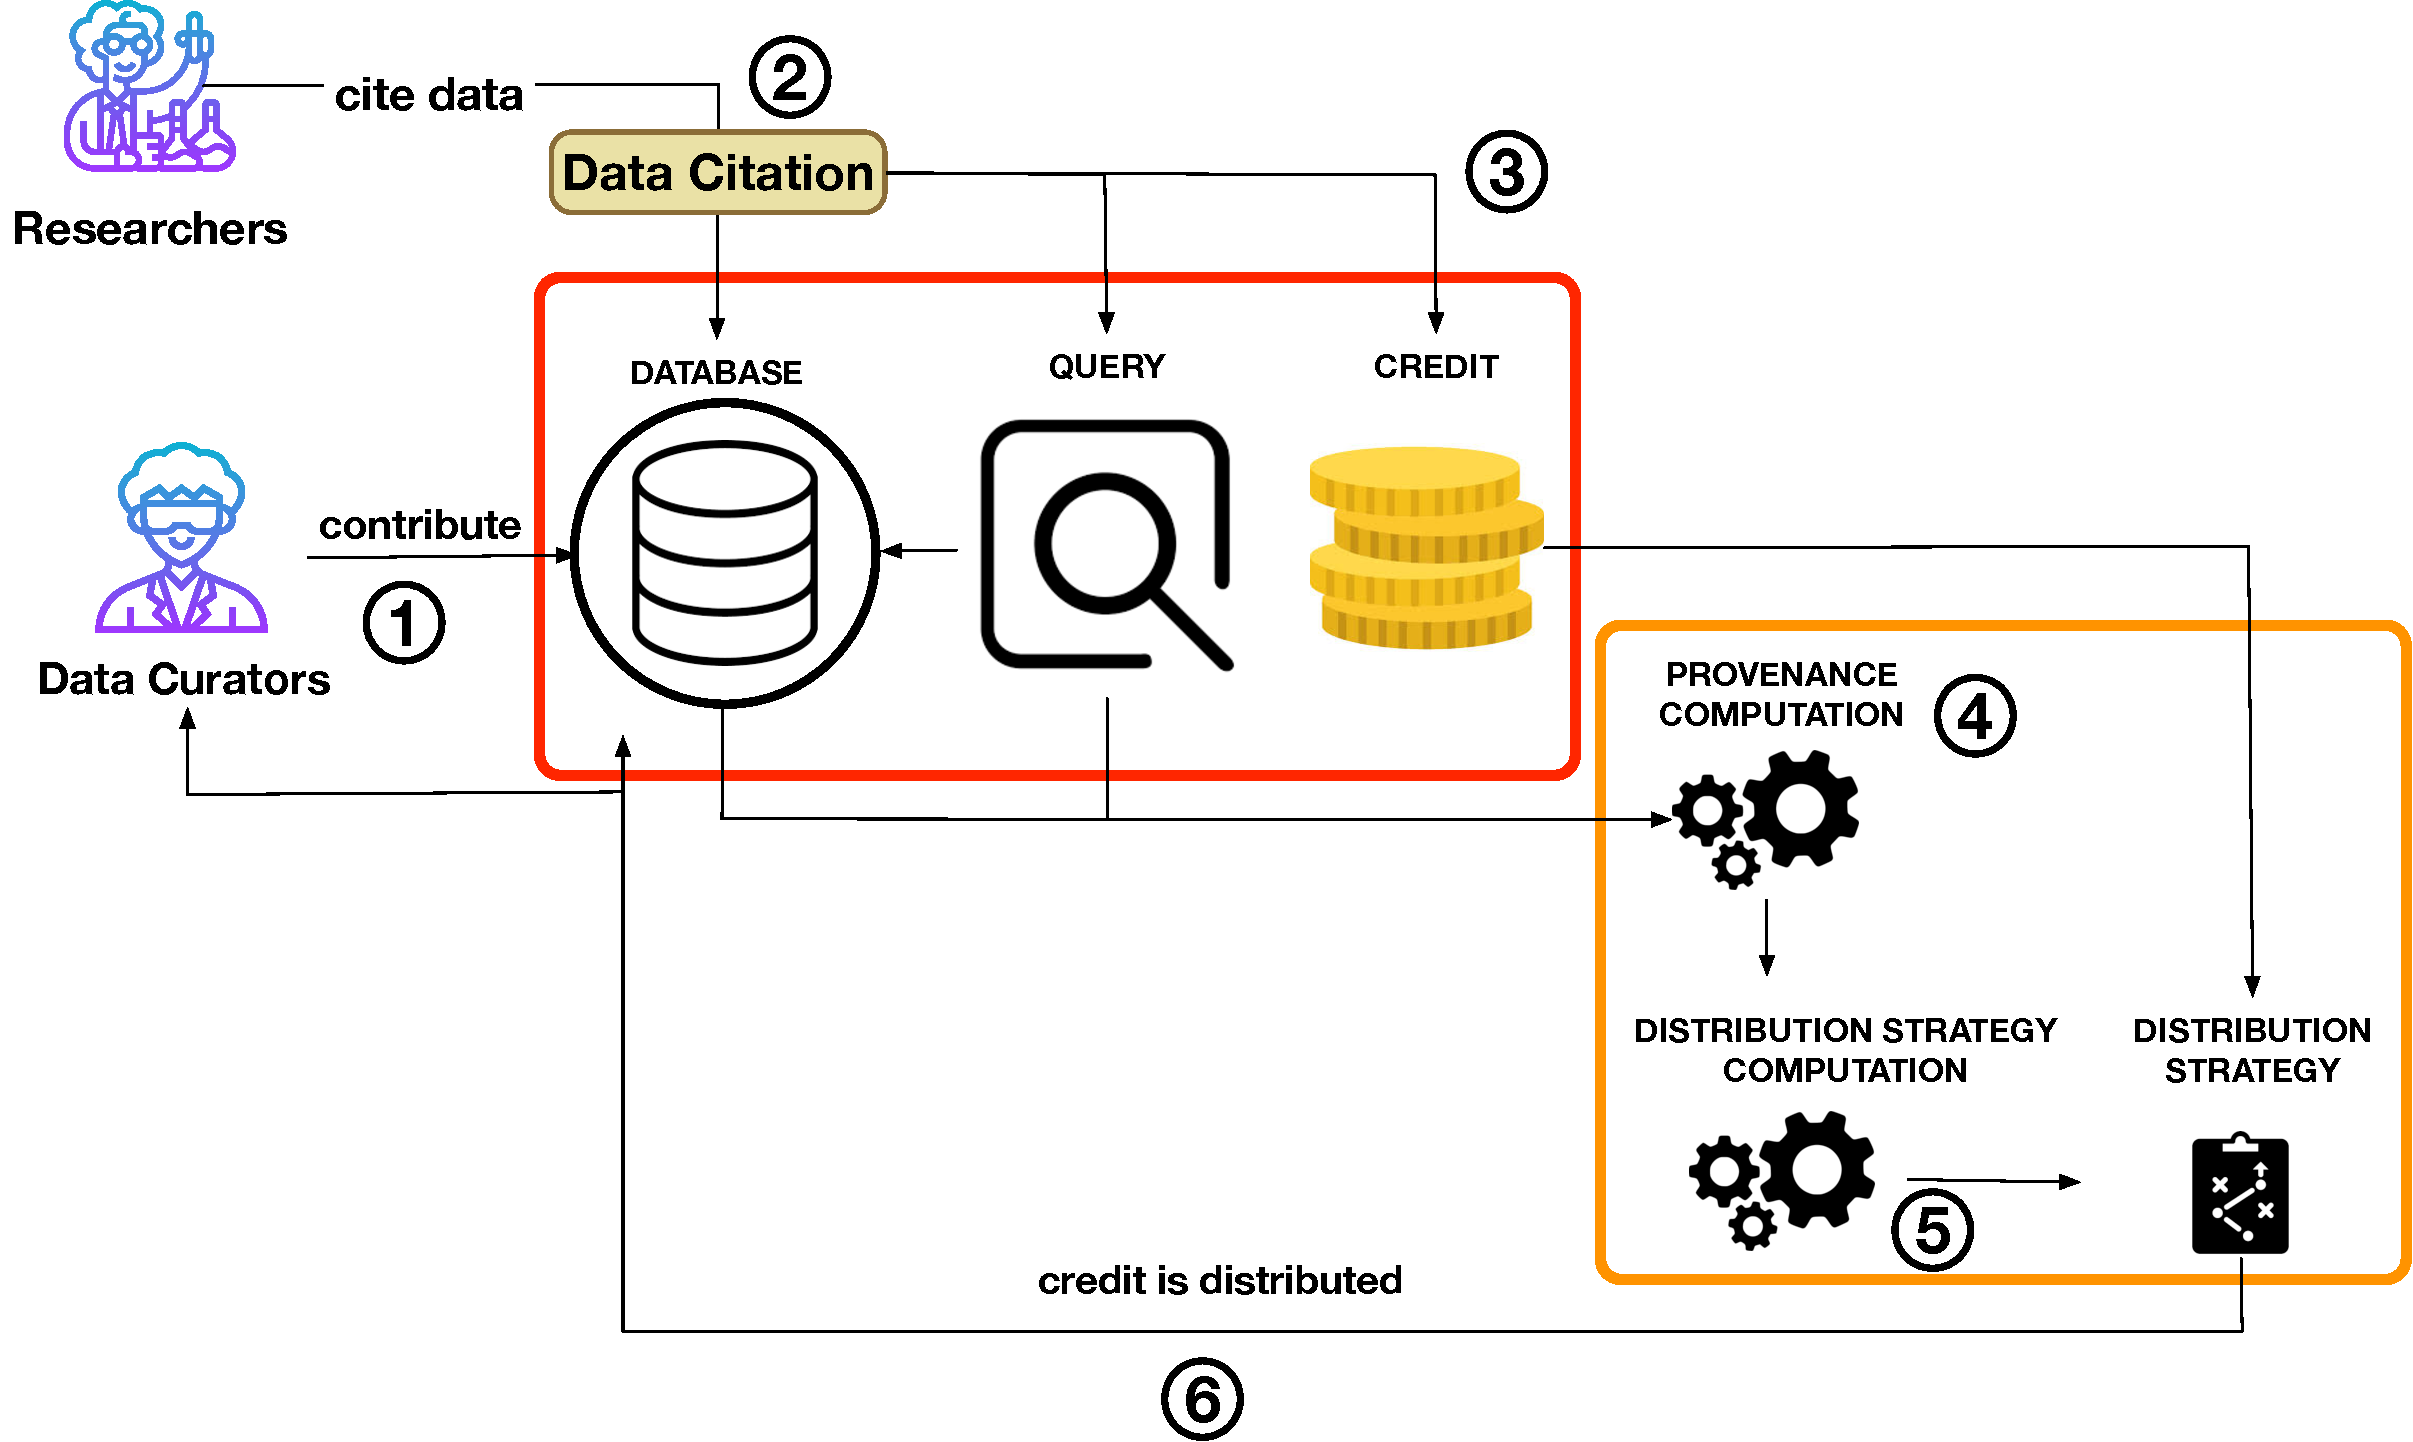
\includegraphics[width=.85\textwidth]{./figures/overview}
    \caption{Overview of the credit distribution pipeline.}
\label{fig:system_overview}
\end{figure}


% \scream{I find the description of this figure confusing. Is the assumption that this is a provenance enabled db which is capable of returning a citation along with the query result? So Step 2 is that the user issues a query that generates the data used, along with the citation?  Step 3 is then assuming the citation is used in a published paper, which generates some credit to the data used.  Step 4 now goes back in time to the db and query at the time it was asked, to calculate the provenance (or perhaps this is stored somehow), which is then used in Step 5 etc. }
\vspace{0.15in}
The DCD process is summarized in Figure \ref{fig:system_overview}:
\vspace{0.15in}
\begin{description}
	\item[Step 1] Scientists and experts contribute 
	the curated information contained in a scientific database.  These are called the ``Data Curators".  
	\item[Step 2] Other researchers use the data in their research, and when possible, cite them. 
% 	\SBD{The rest of this Step is confusing. Rewrote. What dos it matter how researcheers access the data?  and the sentence was not complete.} 
	\item[Step 3] The citation to the data generates credit, that can be used as a proxy for the impact of the data on the citing paper. This credit is represented as a real value $k \in \mathbb{R}_{>0}$. 
	\item[Step 4] Given the database instance $I$ and the query $Q$, it is possible to compute the \emph{data provenance} of $Q(I)$. The provenance of $Q(I)$ is a form of metadata that describes the generation process undertaken by $Q$, and the data used in $I$ to generate the output~\citep{CheneyProvSurvey}. Many different notions of provenance have been proposed in the literature for data in database management systems~\citep{lineageCui, WhyProvBuneman, howProvenanceGreen}, describing different kinds of relationships between data in the input and the output of a query. As reported in \citep{CheneyProvSurvey}, these provenances have been used in several applications beyond giving information on how queries work, for example, annotation propagation and the view update problem. In this paper, we consider three types of provenance: lineage, why-provenance, and how-provenance. \rtwo{Also, we consider ``causality and responsibility''~\cite{MeliouGMS11}, that enrich the information provided by provenance.}
	\item[Step 5] Provenance is input to the DCD problem, whose aim is to compute the \emph{Credit Distribution Strategy} (CDS, also referred only as Distribution Strategy, DS). The CDS is a function $f$ that takes as input the credit value $k $, divides it and distributes it to the data in the input database $I$, and is defined on the basis of citation policies decided at the database administration level or at the domain community level. 
	%Since we are not in a "one-size-fits-all" setting, CDS can be defined with great variability and flexibility, thus allowing for ample customization. 
	In this paper, since we base CDS on data provenance, we describe four CDS, each one based on a different form of provenance. 
	\item[Step 6] Once the CDS is computed, it is used to distribute the given credit $k$ to the parts of the database that are responsible for the generation of $Q(I)$. Transitively, this credit is also divided and given to the corresponding authors of those data.
\end{description}

This paper expands the work in \citep{dosso2020data} %, which addressed the problem of how to reward data and data curators who are typically overlooked in current citation systems.
where we first defined the problem of DCD in relational databases, and proposed a viable Distribution Strategy (DS) based on \emph{lineage} -- the simplest form of \emph{data provenance}.
The lineage of a tuple $t$ in the output $Q(I)$ is defined as the set of all and only the tuples in the database instance $I$ that are ``relevant'' to the production of $t$.
% that is the tuple that are used by $Q$ in the production of $t$.
The corresponding strategy equally redistributes the credit $k$ to the tuples in the lineage set, thus each tuple receives credit $k/|L_t|$, where $L_t$ is the lineage set of $t$. 

One may argue that this DS is too simplistic, since lineage 
%only tells the relevant tuple used to produce the output, and 
does not convey any information about the role or importance of input tuples in the query.
Therefore, one may desire to give more credit to the tuples that are more {\em essential} to the production of the output, i.e. those tuples that, if removed, would prevent the output tuple from appearing in the final result, or those tuples used more than once  by the query. 

Therefore, in this paper, we expand the ideas in \citep{dosso2020data} by proposing three new DSs based on other forms of data provenance: why-provenance~\citep{WhyProvBuneman}, how-provenance~\citep{howProvenanceGreen}, and \rtwo{responsibility~\cite{MeliouGMS11}.} 
\rone{We use these forms of provenance to define new Distribution Strategies that have a different behavior with respect to the one based on lineage} and discuss why one may be preferred to another depending on the application and its goals. 
In particular, we show that why-provenance,  how-provenance and \rtwo{responsibility} are more sensitive to the {\em role} of a tuple in a query, i.e. how many times the tuple is used and how it is used. 
The why-provenance- and \rtwo{responsibility}-based DSs reward more tuples that are essential to the production of the result set, whereas the how-provenance-based DS also takes into consideration the different ways in which a tuple is used. \rone{The newly defined DS strategies exploit the additional information provided by these forms of provenance to weight the contribution of the tuples on the basis of their role in producing the output.  }

The evaluation is based on a well-known curated database, the IUPHAR/BPS\footnote{International Union of Basic and Clinical Pharmacology/British Pharmacology Society} Guide to Pharmacology~\citep{iuphar2018}, also known as GtoPdb\footnote{\url{https://www.guidetopharmacology.org/}}, which contains expertly curated information about diseases, drugs, cellular drug targets, and their mechanisms of action.
We chose GtoPdb for two main reasons: (i) it is a widely-used and valuable curated relational database, (ii) many papers in the literature use, and cite, its data (i.e., families, ligands, and receptors). 
Real queries used in papers can therefore be seen as data citations which, in turn, can be used to assign data credit.

We perform four sets of experiments. In the first one, real queries are extracted from papers published in the British Journal of Pharmacology (BJP), that represent data citations to GtoPdb, and are used to distribute credit in the database using the three different provenance-based DSs. 
%We show how, given the peculiar nature of the queries, the three distributions do not present particular differences in this context and why this is the reason. 
In the second and third experiment we analyze the behavior of the different DS when complex citation queries are employed.
In the fourth set of experiments we use both real and synthetic queries to assess the difference between traditional citation and the notion of credit distribution in terms of rewarding those responsible for the data, e.g. data curators.

\textbf{Contributions}
 of this work include:
\begin{itemize}
    \item \rone{Three new Distribution Strategies based on why-provenance, how-provenance, \rtwo{and responsibility}.}
    \item An in-depth analysis of the effects of credit distribution on real-world curated data and of the differences between the three proposed Distribution Strategies.
    \item A comparison between the behavior of traditional citations and data credit in rewarding data curators.
\end{itemize}

\paragraph{\textbf{Outline}} The rest of the paper is organized as follows:
Section \ref{sec:related} presents the background and related work. Section \ref{section:use_case} describes the GtoPdb use case we adopted. Section \ref{section:preliminaries} briefly presents the forms of provenance used in the paper.  Section \ref{section:distribution_strategies} describes the credit distribution problem and the proposed distribution strategies.  In Section \ref{sec:experiments} we present the experimental evaluation. Finally, Section \ref{section:conclusions} draws some conclusions and outlines future work.

%############


 
